\documentclass[10pt,landscape,a4paper]{article}
\usepackage{multicol}
\usepackage[landscape]{geometry}
\usepackage{hyperref}
\usepackage[utf8]{inputenc}
\usepackage{minted}
\usepackage{venndiagram}
\usepackage{graphicx}
\usepackage{cancel}
\usepackage{wasysym}
\usepackage{amssymb}
\usepackage{stmaryrd}


\geometry{top=1cm,left=1.5cm,right=1cm,bottom=1cm}

% Turn off header and footer
\pagestyle{empty}
 
% Redefine section commands to use less space
\makeatletter
\renewcommand{\section}{\@startsection{section}{1}{0mm}%
                                {-1ex plus -.5ex minus -.2ex}%
                                {0.5ex plus .2ex}%x
                                {\normalfont\large\bfseries}}
\renewcommand{\subsection}{\@startsection{subsection}{2}{0mm}%
                                {-1explus -.5ex minus -.2ex}%
                                {0.5ex plus .2ex}%
                                {\normalfont\small\bfseries}}
\renewcommand{\subsubsection}{\@startsection{subsubsection}{3}{0mm}%
                                {-1ex plus -.5ex minus -.2ex}%
                                {1ex plus .2ex}%
                                {\normalfont\footnotesize\bfseries}}
\renewcommand{\@venn@radius}{4mm}
\renewcommand{\@venn@overlap}{2mm}
\renewcommand{\@venn@vgap}{1mm}
\renewcommand{\@venn@hgap}{1mm}
\makeatother

% Don't print section numbers
\setcounter{secnumdepth}{0}

\setlength{\parindent}{0pt}
\setlength{\parskip}{0pt plus 0.5ex}

\newcommand{\sqljoin}[3]{
\begin{multicols*}{2}
  \begin{venndiagram2sets}
    #1
  \end{venndiagram2sets}
  \vfill\columnbreak
  \hspace{-8em}
  \begin{tabular}{ll}
    x & y \\
    \hline
    #2
  \end{tabular}
\end{multicols*}
\mint{sql}{#3}
}

\newcommand{\sql}[1]{\mintinline{sql}{#1}}



% -----------------------------------------------------------------------

\begin{document}

\footnotesize
\begin{multicols*}{3}


% multicol parameters
% These lengths are set only within the two main columns
%\setlength{\columnseprule}{0.25pt}
\setlength{\premulticols}{1pt}
\setlength{\postmulticols}{1pt}
\setlength{\multicolsep}{1pt}
\setlength{\columnsep}{2pt}

\section{Relationales Modell}

\texttt{Game (\underline{Id} INT PK, Name TEXT UNIQUE, Foo INT REFERENCES TblB)}

\section{Abbildung}
\subsection{1:n/n:n Beziehungen}
1:n via Fremdschlüssel (oder Zwischentabelle mit Attributen), n:n via
Zwischentabelle.
\subsection{Vererbung}
\begin{itemize}
\item{Eine Tabelle für Sub-/Superklasse, mit enum: \\ \sql{CREATE TYPE angtyp AS ENUM ('Chefin', 'Sysadmin')}}
\item{Je eine Tabelle pro Subklasse}
\item{Eine Superklasse-Tabelle mit allen Attributen (\verb!NULL!)}
\end{itemize}

\section{SQL DDL (Data Definition Language)}

\begin{minted}{sql}
CREATE DTABASE foo WITH OWNER = 'bar';
CREATE TABLE Game (
  ArticleID INTEGER PRIMARY KEY,
  Name VARCHAR(300) NOT NULL,
  Date DATE DEFAULT CURRENT_DATE,
  ...  -- ggf. constraints, ohne "ADD CONSTRAINT"
)
\end{minted}

\begin{minted}{sql}
ALTER TABLE Game
  ADD Kuerzel TYPE CHAR;
  ALTER COLUMN Date TYPE STRING;
\end{minted}

\begin{minted}{sql}
ALTER TABLE AbtLeitung
ADD CONSTRAINT fk_AbtLAbt
  FOREIGN KEY (AbtNr) REFERENCES Abteilung (AbtNr)
  -- AbtLeitung wird gelöscht wenn Abteilung gelöscht wird
  ON DELETE CASCADE;

... CHECK (Salaer BETWEEN 1000 and 20000);

CREATE INDEX name ON tbl (col);
  WHERE state = 'N'; -- partiell

PRIMARY KEY, INDEX, UNIQUE

DROP CONSTRAINT fk_AbtLAbt;
\end{minted}

ON DELETE:

\begin{itemize}
  \item \sql{CASCADE}: Tupel mit Fremdschlüssel werden gelöscht
  \item \sql{NO ACTION / RESTRICT}: Fehler/Rollback
  \item \sql{SET NULL}
  \item \sql{SET DEFAULT}
\end{itemize}

\section{SQL DML (Manipulation)}
\begin{minted}{sql}
INSERT INTO abteilung VALUES (1, 'Verkauf');
UPDATE Ang set salaer = 30000 WHERE persnr = 1100;
DELETE FROM Mitarbeiter WHERE Abteilung_ID = 1;
\end{minted}

\columnbreak
\section{SQL DQL (Query)}

\subsection{Select}
\begin{minted}{sql}
 SELECT DISTINCT Wohnort, Name FROM angestellter
 WHERE AbtNr=3 AND Name LIKE '_lorian B%'
 ORDER BY Wohnort ASC, Name DESC;
\end{minted}

\subsubsection{korrelierte Unterabfrage}

\begin{minted}[escapeinside=||]{sql}
SELECT * from Products p WHERE Quantity <
 (SELECT AVG(Quantity) FROM Items s WHERE |\colorbox{yellow}{p.ID}| = s.ID);
\end{minted}

\begin{description}
\item[Projektion]{$\pi_{\mathrm{foo, bar}}(A)$ \\
    \sql{SELECT foo, bar FROM A;}}
\item[Selektion]{$\sigma_{\mathrm{ID < 10}}(A)$ \\
    \sql{SELECT * FROM A WHERE ID < 10;}}
\item[Umbenennung]{$\rho_{\mathrm{foo} \leftarrow \mathrm{bar}}$ \\
  \sql{SELECT foo AS bar FROM ...;}}
\item[Vereinigung]{$A \cup B$ \\
    \sql{SELECT * FROM A UNION [ALL] SELECT * FROM b;}}
\item[Durchschnitt]{$A \cap B$ \\
    \sql{SELECT * FROM A INTERSECT SELECT * FROM b;}}
\end{description}

\subsection{Join ($\bowtie$)}

\texttt{a.x}: 1, 2 \hspace{2em} \texttt{b.y}: 2, 3

\subsubsection{Inner Join}
\sqljoin{\fillACapB}{2 & 2}{SELECT * FROM a INNER JOIN b ON a.x = b.y;}

\subsubsection{Left Join}
\sqljoin{\fillA}{1 & \texttt{NULL} \\ 2 & 2}{SELECT * FROM a LEFT JOIN b ON a.x = b.x;}
right: dito. Mit \sql{WHERE b.x IS NOT NULL}: ohne $A \cap B$

\subsubsection{Outer join}
\sqljoin{\fillA \fillB}{1 & \texttt{NULL} \\ 2 & 2 \\ \texttt{NULL} & 3}{SELECT * FROM a FULL OUTER JOIN b ON a.x = b.x;}

\subsubsection{Andere}
\begin{description}
\item[natural]{Joinen nach gleichnamigen Attributen, Spalten nur 1x im Resultat}
\item[theta]{RelAlg: join-operator $\Theta \in \{<, \leq, =, \geq, >\}$}
\item[equi]{Join mit \verb|colA = colB|}
\end{description}

\subsection{Group By}
\begin{minted}{sql}
SELECT AVG(Lohn) FROM Ang
GROUP BY Abtnr HAVING AVG(Lohn) > 7000;
\end{minted}

Aggregate functions: \sql{COUNT, FIRST, LAST, MAX, MIN, SUM, AVG} \\
\sql{NULL} wird übersprungen/nicht gezählt

\subsection{Window functions}
\begin{minted}{sql}
SELECT abtnr, MAX(salaer) OVER (PARTITION BY abtnr) FROM Ang;
\end{minted}

Tupel werden beibehalten, wir machen nur eine neue Spalte mit dem maximalen
Salär (Wert ggf. wiederholt).

\subsubsection{rank / lead / lag}
\begin{minted}{sql}
SELECT name, preis, rank() OVER(ORDER BY preis DESC)
FROM game LIMIT 5;  -- 5 teuerste Games
\end{minted}

\begin{description}
  \item[lag(val, offset=1, default=NULL)]{Wert von \emph{offset} Reihen vorher
      (\textbf{lead}: Nachher)}
\end{description}

\subsection{Views}
\sql{CREATE VIEW name AS SELECT ...;}

Updatable: Kein \sql{FROM}-Eintrag; kein with, distinct, group by, having,
limit, offset, union, except, intersect; selbige Spalte nicht mehrmals

\subsection{CTE}
\begin{minted}{sql}
WITH tmp AS (SELECT ...) SELECT * FROM tmp;
\end{minted}

Rekursiv:

\begin{minted}{sql}
WITH RECURSIVE cte (spalten) AS
   (Ursprungsselect UNION ALL Rekursionsselect)
SELECT spalten FROM cte WHERE ...;
\end{minted}

Beispiel:

\begin{minted}{sql}
WITH RECURSIVE unter ( persnr, name, chef ) AS
   (SELECT A.persnr, A.name, A.chef FROM angestellter A
    WHERE A.chef = 1010    UNION ALL
    SELECT A.persnr, A.name, A.chef FROM angestellter A
    INNER JOIN unter B on B.persnr = A.chef
) SELECT * FROM unter ORDER BY chef, persnr;
\end{minted}

\subsection{Varia}

\begin{description}
\item[Scalar fns]{\sql{[U/L]CASE}, \sql{MID(n, s, len)}, \sql{LEN}, \sql{ROUND}, $\ldots$}
\item[EXISTS]{\sql{SELECT * FROM a WHERE EXISTS (SELECT ...)};}
\item[ANY/ALL]{\sql{SELECT * FROM a WHERE a.x < ANY (SELECT ...)};}
\item[IN]{\sql{SELECT * FROM a WHERE a.x IN (1, 2);}}
\item[CAST]{\sql{SELECT CAST(CASE WHEN tot IS NULL THEN 1 ELSE 0 END} \\ \sql{AS
      BOOLEAN);} - alternativ: \sql{(tot IS NULL) AS foo;}}
\item[COALESCE]{\sql{COALESCE(n1, n2, "def");}, erster non-NULL Wert}
\item[3-Werte-Logik]{true/false/unknown. Skalarer Ausdruck/Vergleich mit NULL: NULL.}
\item[Alter]{\sql{SELECT ((current_date - gebdat) / 365) AS Alter}}
\end{description}

\section{SQL DCL (Control)}
\begin{minted}{sql}
CREATE ROLE angguest WITH LOGIN PASSWORD 'hunter2'
GRANT INSERT, SELECT ON TABLE "Ang" TO 'angguest';
REVOKE UPDATE ON "Ang" FROM 'angguest';
\end{minted}

\section{Transactions}
\begin{minted}[escapeinside=||]{sql}
BEGIN TRANSACTION |\colorbox{gray}{ISOLATION LEVEL SERIALIZABLE}|;
INSERT INTO Ang (...) VALUES (...);
SAVEPOINT ang_ok;
UPDATE Ang SET ...;
ROLLBACK TO SAVEPOINT ang_ok;
COMMIT TRANSACTION;
\end{minted}


\vfill
\pagebreak

\section{JDBC}
\begin{minted}{java}
try (Connection conn = DriverManager.getConnection(...) {
  try (Statement stmt = conn.createStatement()) {
    ResultSet rs = stmt.executeQuery("select * from ang");
    while (rs.next()) {
      int val = rs.getInt("tel");
      if (rs.wasNull()) continue;
      System.out.printf("foo: %d\n", val); }}}
\end{minted}

\begin{minted}{java}
try (Statement stmt = ...) {
  conn.setAutoCommit(false);
  conn.setTransactionIsolation(
    Connection.TRANSACTION_SERIALIZABLE);
  stmt.addBatch("UPDATE ...");
  int[] rowCount = stmt.executeBatch()
  conn.commit();
} catch (SQLException ex) {
  conn.rollback();
  // ...
}
\end{minted}

\begin{minted}{java}
PreparedSt. stmt = conn.prepareSt.("INSERT ... (?)");
stmt.setString(1, "Kelly");
stmt.addBatch();
stmt.executeBatch()
\end{minted}

\begin{minted}{java}
St. s = c.createStatement(ResultSet.TYPE_SCROLL_INSENSITIVE,
                          ResultSet.CONCUR_UPDATABLE);
rs.first(); rs.updateInt("Age", 100); rs.updateRow();
rs.moveToInsertRow(); rs.updateInt("B", 20); rs.insertRow();
rs.absolute(1); rs.deleteRow();
\end{minted}

\subsection{Treibertypen}
\begin{enumerate}
  \item JDBC-ODBC-Brücke
  \item Native plattformeigene JDBC-Treiber
  \item Universeller JDBC-Treiber (Java)
  \item Direkte Netzwerktreiber (Java)
\end{enumerate}

\subsection{Serialisierbarkeit}
$r_{1}(x)$: T1 liest x / $w_{1}(x)$: T1 schreibt x / $c_{1}$: T1 commit

Konfliktpotential: 2 Transaktionen, write involviert, dasselbe Obj

\newcommand{\ta}[2]{{\color{blue}#1_{1}#2}}
\newcommand{\tb}[2]{{\color{red}#1_{2}#2}}
\newcommand{\tc}[2]{{\color{green}#1_{3}#2}}

\subsubsection{Schedule}
$\tb{r}{(x)}\ta{r}{(x)}\ta{w}{(x)}\tc{r}{(x)}\tc{w}{(x)}\tc{c}{}\tb{w}{(y)}\ta{w}{(y)}\ta{c}{}\tb{c}{}$ \\
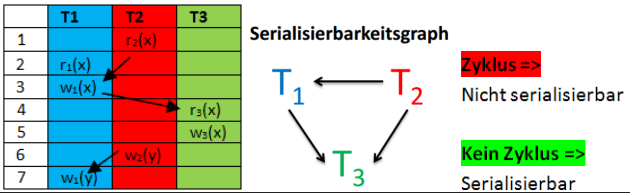
\includegraphics[width=20em]{serial.png}

\subsection{Concurrency-Probleme}
\begin{description}
\item[Lost Update]{$\ta{r}{(x)} \tb{w}{(x)} \ta{w}{(x)}$ (z.B. += 5)}
\item[Dirty Read]{$\ta{w}{(x)} \tb{r}{(x)} \ta{\mathrm{rollback}}{(x)}$}
\item[Non-Repeatable read]{$\ta{r}{(x_{1})} \tb{w}{(x)} \ta{r}{(x_{2})} \rightarrow x_1 \neq x_2$}
\item[Phantom Reads]{$\ta{\mathrm{sel}}{(x_{1})} \tb{\mathrm{ins}}{(y)} \ta{\mathrm{sel}}{(x_{2})} \rightarrow x_1 \neq x_2$}
\item[Read skew]{$\ta{r}{(x)}\tb{w}{(x)}\tb{w}{(y)}\ta{r}{(y)} \rightarrow $ \cancel{constraint}}
\item[Write skew]{$\ta{r}{(x)}\tb{r}{(x)}\ta{r}{(y)}\tb{r}{(y)\tb{w}{(x)\ta{w}{(y)}}} \rightarrow $ \cancel{constraint}}
\end{description}

\subsection{Concurrency Control}
\begin{description}
\item[2PL]{Growing/Shrinking Phase: Zuerst alle locks, dann alle unlocks. Strict: Unlocks ganz am Ende.}
\item[Opfersuche]{Zyklus unterbrechen $\rightarrow$ (ggf. cascading) rollback}
\item[Timestamps/MVCC]{Timestamps $t_x$ und $t_T$. Schreiben: \\ $t_x = t_T$.
    Lesen: $t_x \leq t_T$. Non-blocking reads!}
\item[Validation]{Snapshot, Commit, falls snapshot dirty: rollback}
\item[Deadlock-Voraussetzungen] mutex, geschachtelte locks, zyklisches Warten, locks ohne timeout
\item[Locks] \emph{slock} nur lesend (shared mit reader) \emph{xlock} exklusiv
\item[Optimistisches Locking] Prognose: Wenig writes. Kein slock, aber Zeitstempel prüfen.
\item[Pessimistisches Locking] Prognose: Viel writes. slock und xlock.
\end{description}

\begin{tabular}{lllllll}
  serializable & & \cancel{dead} & \cancel{casc. rb} & \cancel{confl. rb.} & $\parallel$ & real. \\
  \hline
  2PL & \checked & - & - & \checked & - & - \\
  Strict 2PL & \checked & - & \checked & \checked & - & \checked \\
  Preclaiming $\sim$ & \checked & \checked & \checked & \checked & - & -\\
  Validation & \checked & \checked & - & - & \checked & \checked \\
  Timestamp & \checked & \checked & - & - & \checked & \checked \\
  Snapshot & - & \checked PG & \checked & - & \checked & \checked \\
  SSI & \checked & \checked PG & \checked & - & \checked & \checked
\end{tabular}

\subsection{Isolation levels}

\checked: möglich; (-): unmöglich mit cursor stability

\begin{tabular}{lllll}
  Isolation & Dirty & Lost upd. & Nonrep. & Phantom \\
  \hline
  Read uncommited & \checked & (-) & \checked & \checked \\
  \textbf{Read committed} & - & (-) & \checked & \checked \\
  Repeatable read & - & - & - & \checked \\
  Serializable & - & - & - & -
\end{tabular}

\subsection{Fehlerbehandlung}
WAL (write ahead log): Zuerst Log schreiben, dann commit.

Loganalyse $\rightarrow$ Fertige Transaktionen \emph{redo}, angebrochene
Transaktionen \emph{undo}

Loginhalt: [LSN (sequence number), TransaktionsID, PageID, Redo (SQL),
Undo (SQL), PrevLSN]

\section{Btree}

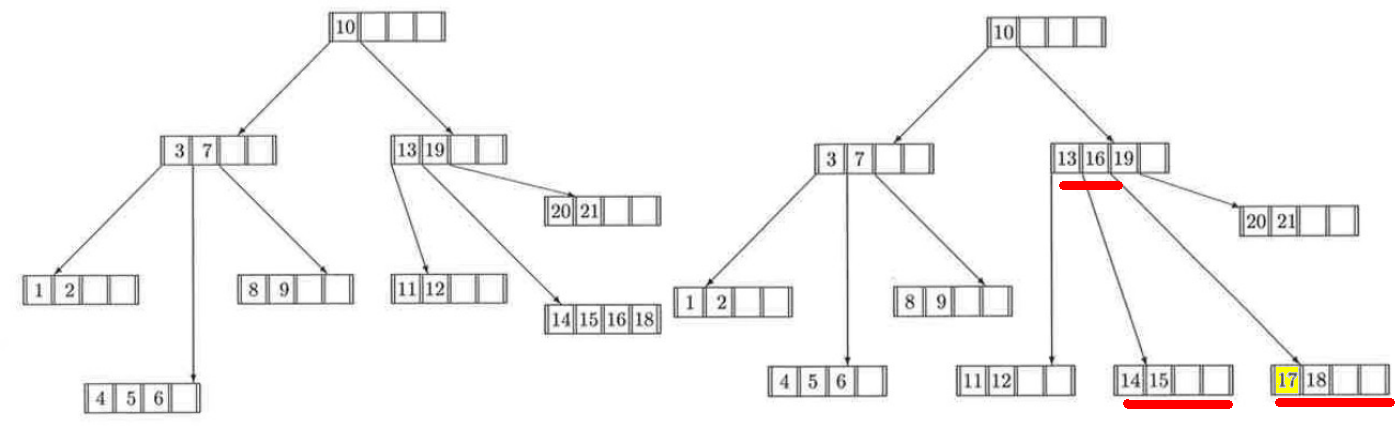
\includegraphics[width=\columnwidth]{bbaum.png}

$k = 2 \Rightarrow k..2k$ keys (ausser root), max. 2k+1 Unterknoten.

\begin{itemize}
  \item Einfügen am Ordnungsplatz
  \item Falls Überlauf: teilen
  \item Neuer Knoten mit Zahlen rechts von mittlerer Zahl
  \item Mitte $\rightarrow$ Vaterknoten
  \item Neuer Knoten mit Vaterknoten verknüpfen
  \item Falls Vaterknoten überfüllt: Neue Root, oder wieder teilen
\end{itemize}

\section{UML}

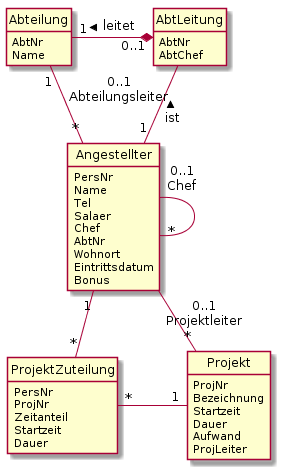
\includegraphics[height=\columnwidth-2em,angle=90]{uml.png}

Typen! Notizen mit Eselsohr-Rechteck und gestricheltem Pfeil.

Diamant oben \textbf{falsch}! Abteilung $\blacklozenge -$ AbtLeitung heisst
``Abt has-a AbtLeitung'' und entspricht \sql{ON DELETE CASCADE} auf Rückseite.

Vererbung mit subclass {\huge$\rightarrowtriangle$} superclass.

\section{Begriffe}

\begin{description}
\item[DBS]{DBMS + $n \cdot \mathrm{DB}$}
\item[Vorteile]{Skalierbar, Permissions, Integrität, Live-Abfragen, Kapslung}
\item[Funktionen]{Transaktionen, Mehrbenutzer, Backups, $\ldots$}
\item[3-Ebenen]{\emph{externe Ebene} (Anwendungen-Sicht), \emph{logische (konzeptionale) Ebene}
    (DB/konzeptionelles Schema, letzteres ist Modell der Realität), \emph{interne
    Ebene}. Durch Trennung: Datenunabhängigkeit}
\item[Datenbasis]{Daten auf HDD - Anwendungsdaten und Data Dictionary (Metadaten)}
\item[Modelle]{Hierarchisch, Netzwerk, Relationen, Postrelational (Methoden,
    nicht mehr 1NF), Objektrelational, OO (Objekte in DB)}
\item[Tier]{\emph{1-Tier}: DBMS im selben Prozess wie Client (MS Access), \emph{2-Tier}:
    gleiche Maschine}
\item[Entitätstyp]{Klasse}
\item[Schlüsselkandidaten]{Minimale Attributskombinationen, die eine Entität
    gerade noch eindeutig identifizieren}
\item[1.NF]{Wertebereiche der Tabelle sind atomar (z.B. nicht Vor-/Nachname in 1 Attribut)}
\item[2.NF]{Tabelle mit mehreren Primärschlüsselattributen: Nichtschlüsselattr. sind
    von jedem Schlüsselattr. abhängig}
\item[3.NF]{2.NF mit Transitivität ($A \leftarrow C$ wenn $A \leftarrow B \leftarrow C$)}
\item[ACID]{Atomicity, Consistency, Isolation, Durability}
\item[Indexe]{ISAM (Aufsteigend via Indexspalte, überlaufseiten möglich), Hash, BRIN, GiST, GIN, Btree, Bitmap. Kann funktional/zusammengesetzt/partiell/clustered sein.}
\item[Mutationsanomalien]{Bei Redundanz. INSERT-, UPDATE-, DELETE-Anomalie}
\item[Surrogatschlüssel]{Künstlicher Schlüssel, z.B. für Performance bei
    zusammengesetztem Schlüssel}.
\end{description}


\end{multicols*}
\end{document}
